% Generated by pysimcount.pfchilds -- do not edit; regenerate instead.
% figure: grouping-cnot-twogroup-odd-out -- Every formula, two-group grouping (twogroup-odd-out), cnot gates vs n (even n only)
% source: ../np-grouping/aggregate.json (seeds [1, 2, 3, 4, 5, 6, 7, 8, 9, 10]); run commits: 01d3c275ceae2840002bd1aaea68f59b987c4975
% metric=cnot kind=twogroup-odd-out merged (cz, simcount template)
% measured n: mean over seeds of the run's totals; bars min..max over seeds
% r from power-law fit to mean measured r (n = 6--10); r = ceil(a n^b); point=mean-r-fit; bars = min..max of per-seed fits
% per-step counts exactly affine in n (checked on n = [10, 20, 40], direct build at n = [100])
% shown: suzuki4, suzuki6, mo-q6, mo-q14, bm-q10, mo-o8-q21, morales-y8m10, morales-m8
% removed (see grouping-cnot-twogroup-odd-out-ranking.md): lie-trotter, suzuki2, suzuki8
% figure made at git_commit=e5d9ee696f892e28aced765585653760f8a427c4 git_dirty=False
% derived: grouping-cnot-twogroup-odd-out.tex restyled by pysimcount.figuniform: extrapolated points (r from power-law fit) drawn in their series' measured style, style-key legend entries removed; extrapolated n = [14, 20, 30, 50, 70, 100, 200, 300, 500]; source_sha256=9cc92b75b41d8fb155c2f7da1765c7320ca7135cd88cea73837c07c7dc276017
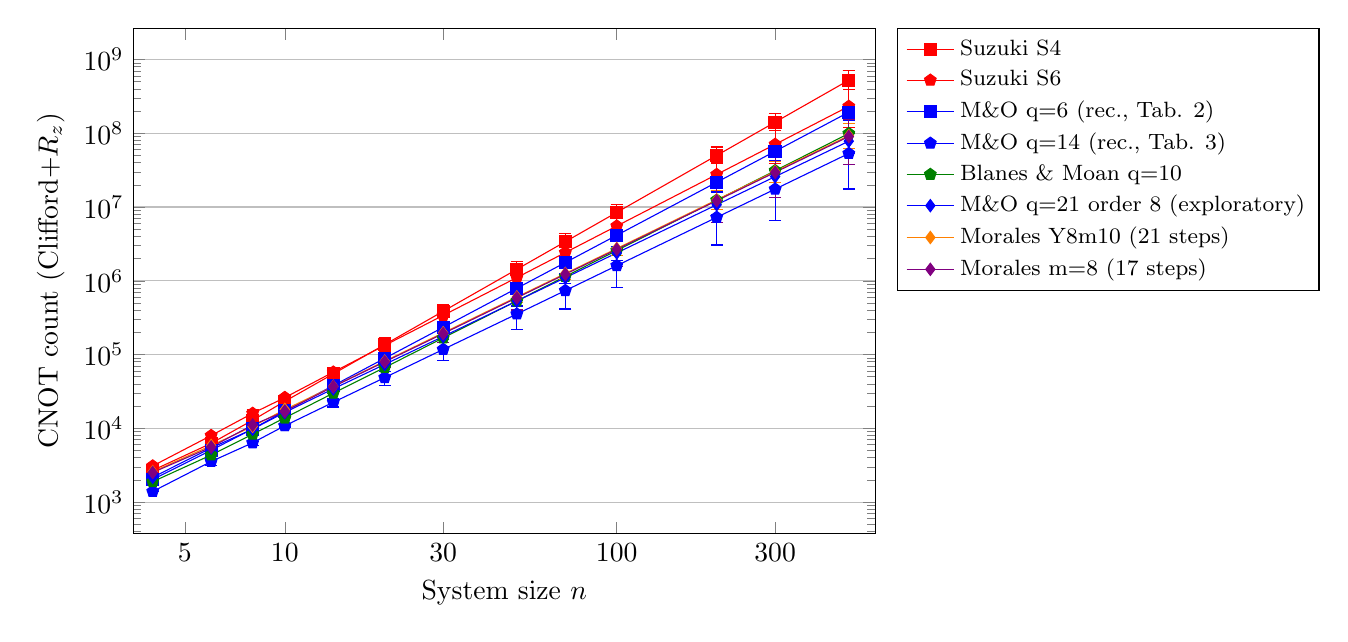
\begin{tikzpicture}
  \begin{loglogaxis}[
    width=11cm, height=8cm,
    xlabel={System size $n$},
    ylabel={CNOT count (Clifford+$R_z$)},
    xtick={5,10,30,100,300}, xticklabels={5,10,30,100,300},
    xmin=3.5, xmax=600,
    ymajorgrids=true,
    legend pos=outer north east,
    legend cell align=left,
    legend style={font=\footnotesize},
  ]
    % suzuki4: measured n, mean over seeds, bars min..max over seeds
    \addplot[red, solid, mark=square*, mark size=2.2pt, mark options={solid, fill=red}, error bars/.cd, y dir=both, y explicit, error bar style={solid}] coordinates {
      (4,2692.8) += (0,79.2) -= (0,52.8)
      (6,6256.8) += (0,79.2) -= (0,118.8)
      (8,12883.2) += (0,580.8) -= (0,475.2)
      (10,23215.5) += (0,874.5) -= (0,775.5)
    };
    \addlegendentry{Suzuki S4}
    % suzuki4: extrapolated, r = ceil(3.81587 n^1.56408), per step = 33/2 n + 0; bars min..max of per-seed fits
    \addplot[red, solid, mark=square*, mark size=2.2pt, mark options={solid, fill=red}, forget plot, error bars/.cd, y dir=both, y explicit, error bar style={solid}] coordinates {
      (10,23215.5)
      (14,54747) += (0,2772) -= (0,2310)
      (20,136620) += (0,10560) -= (0,8910)
      (30,386100) += (0,42075) -= (0,35640)
      (50,1.43055e+06) += (0,216150) -= (0,180675)
      (70,3.38992e+06) += (0,607530) -= (0,500115)
      (100,8.4579e+06) += (0,1.78035e+06) -= (0,1.4322e+06)
      (200,5.00181e+07) += (0,1.36488e+07) -= (0,1.05204e+07)
      (300,1.41456e+08) += (0,4.39906e+07) -= (0,3.30066e+07)
      (500,5.24156e+08) += (0,1.88999e+08) -= (0,1.36991e+08)
    };
    % suzuki6: measured n, mean over seeds, bars min..max over seeds
    \addplot[red, solid, mark=pentagon*, mark size=2.2pt, mark options={solid, fill=red}, error bars/.cd, y dir=both, y explicit, error bar style={solid}] coordinates {
      (4,3090.6) += (0,275.4) -= (0,30.6)
      (6,7986.6) += (0,275.4) -= (0,642.6)
      (8,15973.2) += (0,1774.8) -= (0,1897.2)
      (10,26086.5) += (0,1453.5) -= (0,841.5)
    };
    \addlegendentry{Suzuki S6}
    % suzuki6: extrapolated, r = ceil(1.64274 n^1.32149), per step = 153/2 n + 0; bars min..max of per-seed fits
    \addplot[red, solid, mark=pentagon*, mark size=2.2pt, mark options={solid, fill=red}, forget plot, error bars/.cd, y dir=both, y explicit, error bar style={solid}] coordinates {
      (10,26086.5)
      (14,57834) += (0,9639) -= (0,6426)
      (20,133110) += (0,35190) -= (0,22950)
      (30,339660) += (0,142290) -= (0,73440)
      (50,1.10542e+06) += (0,699975) -= (0,302175)
      (70,2.4151e+06) += (0,1.90638e+06) -= (0,749700)
      (100,5.53095e+06) += (0,5.355e+06) -= (0,1.92015e+06)
      (200,2.76165e+07) += (0,3.80358e+07) -= (0,1.13526e+07)
      (300,7.07778e+07) += (0,1.17022e+08) -= (0,3.15792e+07)
      (500,2.3168e+08) += (0,4.74224e+08) -= (0,1.12914e+08)
    };
    % mo-q6: measured n, mean over seeds, bars min..max over seeds
    \addplot[blue, solid, mark=square*, mark size=2.2pt, mark options={solid, fill=blue}, error bars/.cd, y dir=both, y explicit, error bar style={solid}] coordinates {
      (4,2028) += (0,0) -= (0,0)
      (6,5042.7) += (0,105.3) -= (0,11.7)
      (8,9828) += (0,0) -= (0,0)
      (10,17101.5) += (0,253.5) -= (0,331.5)
    };
    \addlegendentry{M\&O q=6 (rec., Tab. 2)}
    % mo-q6: extrapolated, r = ceil(3.56738 n^1.38733), per step = 39/2 n + 0; bars min..max of per-seed fits
    \addplot[blue, solid, mark=square*, mark size=2.2pt, mark options={solid, fill=blue}, forget plot, error bars/.cd, y dir=both, y explicit, error bar style={solid}] coordinates {
      (10,17101.5)
      (14,37947) += (0,1092) -= (0,819)
      (20,88920) += (0,3120) -= (0,3120)
      (30,234000) += (0,11115) -= (0,11115)
      (50,791700) += (0,52650) -= (0,50700)
      (70,1.76768e+06) += (0,136500) -= (0,131040)
      (100,4.1418e+06) += (0,372450) -= (0,351000)
      (200,2.16645e+07) += (0,2.4804e+06) -= (0,2.262e+06)
      (300,5.70316e+07) += (0,7.3593e+06) -= (0,6.6105e+06)
      (500,1.93079e+08) += (0,2.85285e+07) -= (0,2.5194e+07)
    };
    % mo-q14: measured n, mean over seeds, bars min..max over seeds
    \addplot[blue, solid, mark=pentagon*, mark size=2.2pt, mark options={solid, fill=blue}, error bars/.cd, y dir=both, y explicit, error bar style={solid}] coordinates {
      (4,1392) += (0,0) -= (0,0)
      (6,3549.6) += (0,365.4) -= (0,417.6)
      (8,6368.4) += (0,243.6) -= (0,452.4)
      (10,10831.5) += (0,478.5) -= (0,391.5)
    };
    \addlegendentry{M\&O q=14 (rec., Tab. 3)}
    % mo-q14: extrapolated, r = ceil(1.63049 n^1.17678), per step = 87/2 n + 0; bars min..max of per-seed fits
    \addplot[blue, solid, mark=pentagon*, mark size=2.2pt, mark options={solid, fill=blue}, forget plot, error bars/.cd, y dir=both, y explicit, error bar style={solid}] coordinates {
      (10,10831.5)
      (14,22533) += (0,2436) -= (0,3045)
      (20,48720) += (0,10440) -= (0,10440)
      (30,117450) += (0,40455) -= (0,33930)
      (50,354525) += (0,193575) -= (0,134850)
      (70,736890) += (0,505470) -= (0,322770)
      (100,1.60515e+06) += (0,1.35285e+06) -= (0,787350)
      (200,7.2471e+06) += (0,8.7435e+06) -= (0,4.1847e+06)
      (300,1.75e+07) += (0,2.54344e+07) -= (0,1.08576e+07)
      (500,5.32005e+07) += (0,9.57652e+07) -= (0,3.56265e+07)
    };
    % bm-q10: measured n, mean over seeds, bars min..max over seeds
    \addplot[green!50!black, solid, mark=pentagon*, mark size=2.2pt, mark options={solid, fill=green!50!black}, error bars/.cd, y dir=both, y explicit, error bar style={solid}] coordinates {
      (4,1890) += (0,0) -= (0,0)
      (6,4347) += (0,0) -= (0,0)
      (8,8316) += (0,0) -= (0,0)
      (10,13860) += (0,0) -= (0,0)
    };
    \addlegendentry{Blanes \& Moan q=10}
    % bm-q10: extrapolated, r = ceil(2.36355 n^1.26919), per step = 63/2 n + 0; bars min..max of per-seed fits
    \addplot[green!50!black, solid, mark=pentagon*, mark size=2.2pt, mark options={solid, fill=green!50!black}, forget plot, error bars/.cd, y dir=both, y explicit, error bar style={solid}] coordinates {
      (10,13860)
      (14,29988) += (0,0) -= (0,0)
      (20,66780) += (0,0) -= (0,0)
      (30,168210) += (0,0) -= (0,0)
      (50,533925) += (0,0) -= (0,0)
      (70,1.1466e+06) += (0,0) -= (0,0)
      (100,2.57355e+06) += (0,0) -= (0,0)
      (200,1.23984e+07) += (0,0) -= (0,0)
      (300,3.11188e+07) += (0,0) -= (0,0)
      (500,9.91778e+07) += (0,0) -= (0,0)
    };
    % mo-o8-q21: measured n, mean over seeds, bars min..max over seeds
    \addplot[blue, solid, mark=diamond*, mark size=2.2pt, mark options={solid, fill=blue}, error bars/.cd, y dir=both, y explicit, error bar style={solid}] coordinates {
      (4,2167.2) += (0,154.8) -= (0,103.2)
      (6,5418) += (0,387) -= (0,387)
      (8,9752.4) += (0,567.6) -= (0,464.4)
      (10,16447.5) += (0,967.5) -= (0,322.5)
    };
    \addlegendentry{M\&O q=21 order 8 (exploratory)}
    % mo-o8-q21: extrapolated, r = ceil(1.70915 n^1.16766), per step = 129/2 n + 0; bars min..max of per-seed fits
    \addplot[blue, solid, mark=diamond*, mark size=2.2pt, mark options={solid, fill=blue}, forget plot, error bars/.cd, y dir=both, y explicit, error bar style={solid}] coordinates {
      (10,16447.5)
      (14,34314) += (0,4515) -= (0,1806)
      (20,73530) += (0,16770) -= (0,5160)
      (30,176085) += (0,63855) -= (0,17415)
      (50,532125) += (0,293475) -= (0,77400)
      (70,1.10166e+06) += (0,758520) -= (0,194145)
      (100,2.3865e+06) += (0,2.01885e+06) -= (0,490200)
      (200,1.07328e+07) += (0,1.2771e+07) -= (0,2.7993e+06)
      (300,2.58322e+07) += (0,3.67844e+07) -= (0,7.52715e+06)
      (500,7.81418e+07) += (0,1.3703e+08) -= (0,2.55742e+07)
    };
    % morales-y8m10: measured n, mean over seeds, bars min..max over seeds
    \addplot[orange, solid, mark=diamond*, mark size=2.2pt, mark options={solid, fill=orange}, error bars/.cd, y dir=both, y explicit, error bar style={solid}] coordinates {
      (4,2580) += (0,0) -= (0,0)
      (6,5843.7) += (0,348.3) -= (0,38.7)
      (8,10629.6) += (0,206.4) -= (0,309.6)
      (10,17931) += (0,774) -= (0,516)
    };
    \addlegendentry{Morales Y8m10 (21 steps)}
    % morales-y8m10: extrapolated, r = ceil(1.77538 n^1.18938), per step = 129/2 n + 0; bars min..max of per-seed fits
    \addplot[orange, solid, mark=diamond*, mark size=2.2pt, mark options={solid, fill=orange}, forget plot, error bars/.cd, y dir=both, y explicit, error bar style={solid}] coordinates {
      (10,17931)
      (14,37023) += (0,2709) -= (0,903)
      (20,81270) += (0,7740) -= (0,5160)
      (30,197370) += (0,25155) -= (0,19350)
      (50,603075) += (0,106425) -= (0,90300)
      (70,1.25517e+06) += (0,270900) -= (0,216720)
      (100,2.74125e+06) += (0,690150) -= (0,561150)
      (200,1.25001e+07) += (0,4.128e+06) -= (0,3.225e+06)
      (300,3.03602e+07) += (0,1.14939e+07) -= (0,8.7462e+06)
      (500,9.288e+07) += (0,4.1022e+07) -= (0,3.00892e+07)
    };
    % morales-m8: measured n, mean over seeds, bars min..max over seeds
    \addplot[violet, solid, mark=diamond*, mark size=2.2pt, mark options={solid, fill=violet}, error bars/.cd, y dir=both, y explicit, error bar style={solid}] coordinates {
      (4,2520) += (0,0) -= (0,0)
      (6,5575.5) += (0,409.5) -= (0,220.5)
      (8,11088) += (0,252) -= (0,168)
      (10,16957.5) += (0,367.5) -= (0,682.5)
    };
    \addlegendentry{Morales m=8 (17 steps)}
    % morales-m8: extrapolated, r = ceil(2.14576 n^1.18752), per step = 105/2 n + 0; bars min..max of per-seed fits
    \addplot[violet, solid, mark=diamond*, mark size=2.2pt, mark options={solid, fill=violet}, forget plot, error bars/.cd, y dir=both, y explicit, error bar style={solid}] coordinates {
      (10,16957.5)
      (14,36750) += (0,2940) -= (0,3675)
      (20,79800) += (0,9450) -= (0,13650)
      (30,192150) += (0,36225) -= (0,45675)
      (50,588000) += (0,154875) -= (0,186375)
      (70,1.22745e+06) += (0,389550) -= (0,452025)
      (100,2.67225e+06) += (0,1.01325e+06) -= (0,1.1025e+06)
      (200,1.218e+07) += (0,6.132e+06) -= (0,6.0375e+06)
      (300,2.9547e+07) += (0,1.72148e+07) -= (0,1.58918e+07)
      (500,9.03262e+07) += (0,6.20812e+07) -= (0,5.29725e+07)
    };
  \end{loglogaxis}
\end{tikzpicture}
